%%%%%%%%%%%%%%%%%%%%%%%%%%%%%%%%%%%%%%%%%
% Journal Article
% LaTeX Template
% Version 1.4 (15/5/16)
%
% This template has been downloaded from:
% http://www.LaTeXTemplates.com
%
% Original author:
% Frits Wenneker (http://www.howtotex.com) with extensive modifications by
% Vel (vel@LaTeXTemplates.com)
%
% License:
% CC BY-NC-SA 3.0 (http://creativecommons.org/licenses/by-nc-sa/3.0/)
%
%%%%%%%%%%%%%%%%%%%%%%%%%%%%%%%%%%%%%%%%%

%----------------------------------------------------------------------------------------
%	PACKAGES AND OTHER DOCUMENT CONFIGURATIONS
%----------------------------------------------------------------------------------------

\documentclass[twoside,twocolumn, 11pt]{article}
\usepackage[english, russian]{babel}
\usepackage{graphicx}
\graphicspath{{Materials/graphics/}{Materials/graphs/}{Materials/}}  % папки с картинками
\usepackage[utf8]{inputenc}
\usepackage{blindtext} % Package to generate dummy text throughout this template
\usepackage{xcolor}
\usepackage[T1,T2A]{fontenc}

\usepackage[sc]{mathpazo} % Use the Palatino font
\usepackage[T1]{fontenc} % Use 8-bit encoding that has 256 glyphs
\linespread{1.05} % Line spacing - Palatino needs more space between lines
\usepackage{microtype} % Slightly tweak font spacing for aesthetics

\usepackage[english]{babel} % Language hyphenation and typographical rules

\usepackage[hmarginratio=1:1, top=25mm, columnsep=33pt]{geometry} % Document margins
\usepackage[hang, small,labelfont=bf,up,textfont=it,up]{caption} % Custom captions under/above floats in tables or figures
\usepackage{booktabs} % Horizontal rules in tables

\usepackage{lettrine} % The lettrine is the first enlarged letter at the beginning of the text

\usepackage{enumitem} % Customized lists
\setlist[itemize]{noitemsep} % Make itemize lists more compact

\usepackage{abstract} % Allows abstract customization
\renewcommand{\abstractnamefont}{\normalfont\bfseries} % Set the "Abstract" text to bold
\renewcommand{\abstracttextfont}{\normalfont\small\itshape} % Set the abstract itself to small italic text

\usepackage{titlesec} % Allows customization of titles
\renewcommand\thesection{\Roman{section}} % Roman numerals for the sections
\renewcommand\thesubsection{\roman{subsection}} % roman numerals for subsections
\titleformat{\section}[block]{\large\scshape\centering}{\thesection.}{1em}{} % Change the look of the section titles
\titleformat{\subsection}[block]{\large}{\thesubsection.}{1em}{} % Change the look of the section titles

\usepackage{fancyhdr} % Headers and footers
\pagestyle{fancy} % All pages have headers and footers
\fancyhead{} % Blank out the default header
\fancyfoot{} % Blank out the default footer
\fancyhead[C]{Моделирование идеального газа $\bullet$ Январь 2020 $\bullet$ МФТИ} % Custom header text
\fancyfoot[RO, LE]{\thepage} % Custom footer text

\usepackage{geometry} % Простой способ задавать поля
\geometry{top=25mm}
\geometry{bottom=30mm}
% \geometry{left=25mm}
% \geometry{right=25mm}

\usepackage{titling} % Customizing the title section
\usepackage{comment} % Для комментирования

\usepackage{hyperref} % For hyperlinks in the PDF
\usepackage{amssymb,amsmath,amsthm}

\usepackage{mathtools}

\theoremstyle{plain}
\newtheorem{theorem}{Теорема}
\newtheorem{lemma}{Лемма}
\newtheorem{proposition}{Утверждение}
\newtheorem{corollary}{Следствие}
\newtheorem{conclusion}{Вывод}
\theoremstyle{definition}
\newtheorem{definition}{Определение}
\newtheorem{notation}{Обозначение}
\newtheorem{example}{Пример}
\DeclareMathOperator{\sign}{sign}

\DeclarePairedDelimiter\abs{\lvert}{\rvert} %палочки модуля

%----------------------------------------------------------------------------------------
%	TITLE SECTION
%----------------------------------------------------------------------------------------

\setlength{\droptitle}{-4\baselineskip} % Move the title up

\pretitle{\begin{center} \Huge\bfseries} % Article title formatting
\posttitle{\end{center}} % Article title closing formatting
\title{Компьютерное моделирование идеального газа, распределение Максвелла, флуктуации.} % Article title
\author{%
\textsc{Н. В. Павличенко, А. С. Подкидышев} \\[1ex] % Your name
\normalsize Московский физико-технический институт \\ % Your institution
\normalsize \href{mailto:pavlichenko.nv@phystech.edu}{pavlichenko.nv@phystech.edu}
\href{mailto:pavlichenko.nv@phystech.edu}{podkidishev.as@phystech.edu}% Your email address
}
%\and % Uncomment if 2 authors are required, duplicate these 4 lines if more
%\textsc{Jane Smith}\thanks{Corresponding author} \\[1ex] % Second author's name
%\normalsize University of Utah \\ % Second author's institution
%\normalsize \href{mailto:jane@smith.com}{jane@smith.com} % Second author's email address

\date{\today} % Leave empty to omit a date
\renewcommand{\maketitlehookd}{%
\begin{abstract}
\noindent В данной статье рассматривается компьютерная модель идеального газа, проверяются некоторые основные законы термодинамики: уравнение Менделеева-Клайперона, распределение Максвелла, закон Бойля-Мариотта, нормальность флуктуаций.
Особенности данной работы в том, что используется трехмерная модель газа, что уже редкость среди существуствующих проектов, а так же в том, что используются реальные параметры газов: масса молекулы и скорость.
\end{abstract}
}

%----------------------------------------------------------------------------------------

%  ToDO
% 1. запустить Spell Checker.
% 2. Разместить ссылку на гитхаб в начале дока.
\begin{document}

% Print the title
\maketitle
%----------------------------------------------------------------------------------------
%	ARTICLE CONTENTS
%----------------------------------------------------------------------------------------
\section{Введение}

\indent Идеальным газом называют такой газ, у которого взаимодействием молекул между собой можно пренебречь. Иначе говоря, это газ,
средняя кинетическая энергия которого много больше энергии их взаимодействия. Например, разряженный газ нейтральных частиц можно считать идеальным.
В курсе общей физики основные законы были рассмотрены со статистической стороны, то есть не затрагивали конкретные микросостояния системы,
а использовали различные усреднения и интуитивные предположения. С другой стороны интересно посмотреть действительно ли это верно, честно просимулировав все состояния
системы с помощью классической механики.

%------------------------------------------------
\section{Цель работы}

% ToDO : поменять в финальной версии(в самом конце)
\begin{enumerate}
\item Связь макро- и микропараметров.
\item Проверить выполнение уравнения состояния идеального газа.
\item Проверить зависимость распределения скоростей от времени (сравнить с распределением Максвелла).
\item Оценить флуктуацию давления. Сравнить с теоретическими предположениями.
\item Просимулировать цикл тепловой машины. Проверить уравниения адиабаты и изотермы.
\end{enumerate}

\section{Описание построенной модели}

\indent Будем считать молекулы твердыми шариками, которые упруго сталкиваются друг с другом и с теплонепроводящими стенками кубического сосуда $1 \times 1 \times 1$ м.
В начале эксперимента будем запускать частицы с одинаковой скоростью и равномерно распределенными направлениями. После этого молекулы будут
соударяться друг с другом и со стенками сосуда. Будем параллельно строить распределение модулей их скоростей, давление и температуру.
\begin{figure}[!h]
    {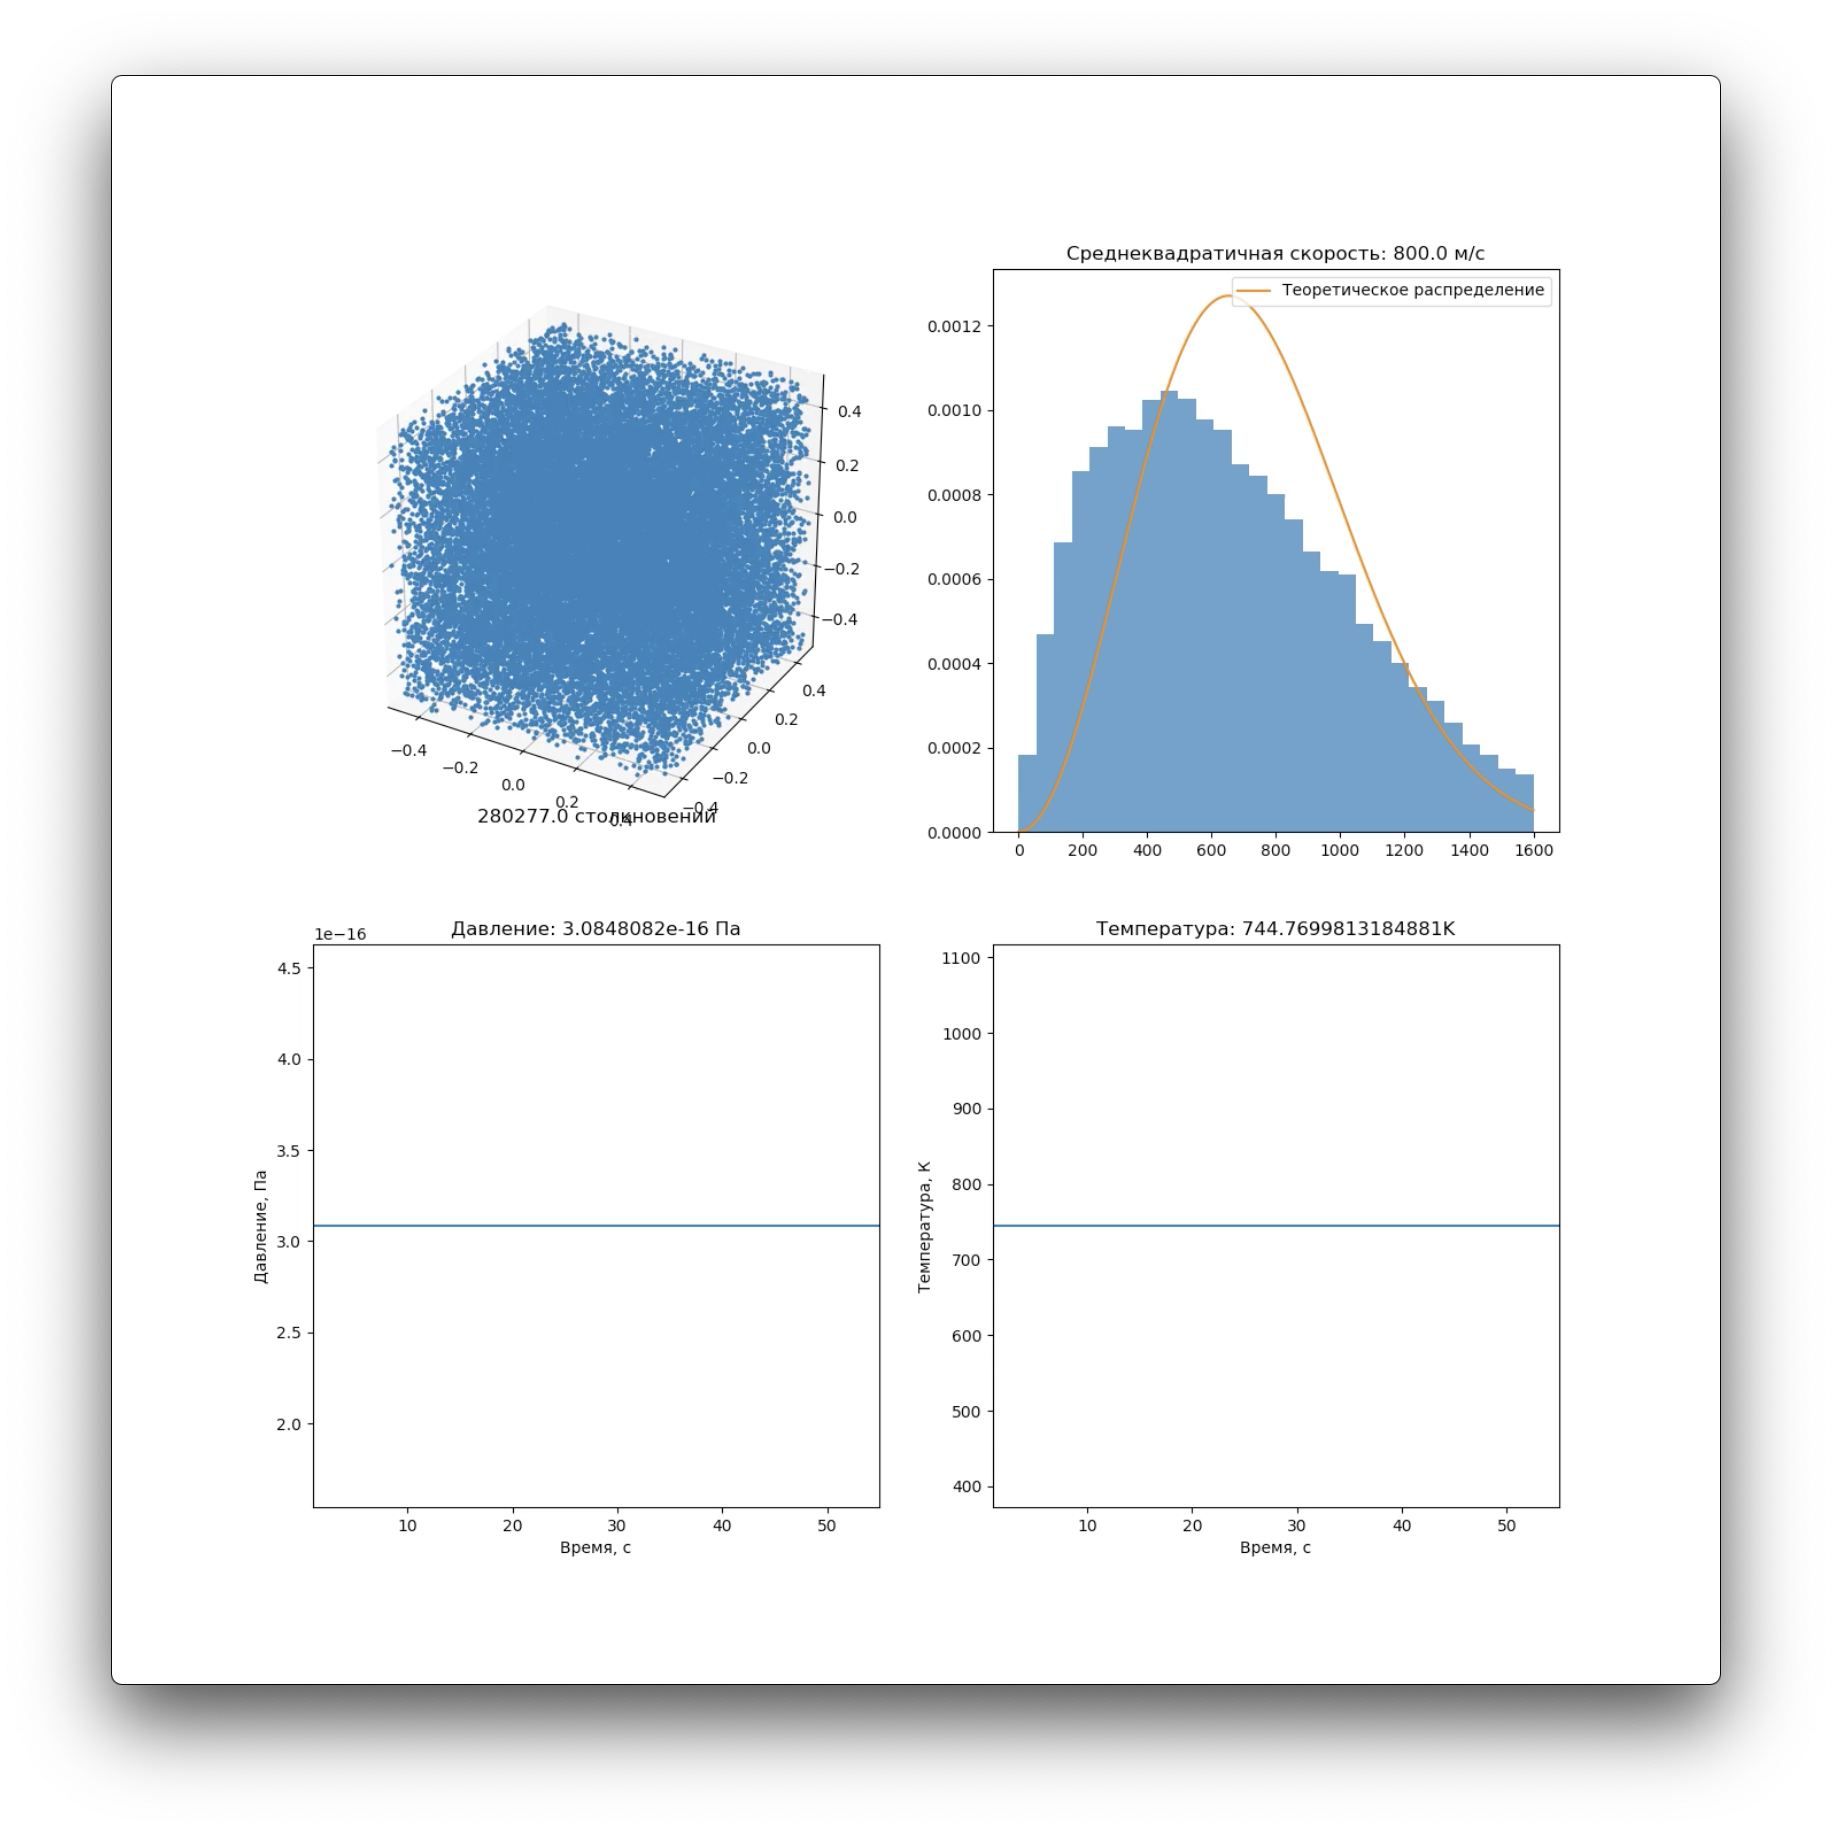
\includegraphics[width=1\linewidth]{ui.png}}
    \caption{Результат симуляции}
\end{figure}
Расчеты проводим на движке, написанном на C++, визуализируем с помощью анимации на Python.

\subsection{Соударение молекул друг с другом}
\indent Критически важной выглядит задача обработки соударений частиц, так как именно от точности этого алгоритма будет зависеть установление распределений скоростей, энергий, и других параметров системы.
Для этого воспользуемся задачей об угле рассеивания при налете одного шара на другой.

Сначала перейдем в систему отсчета второй молекулы (до удара). Тогда в ней вторая частица будет неподвижна и мы сможем свести задачу к обозначенной выше. Теперь перейдем к системе отсчета центра масс. Итоговый вектор перехода равен
\begin{equation}
\vec{W} = \vec{v_2} + \dfrac{1}{2}\vec{v_1}.
\end{equation}
\indent Скорость первой молекулы в новой системе координат тогда $\vec{v}$.
Теперь построим ортонормированный базис в плоскости соударения. Пусть $\vec{x} = \dfrac{\vec{v}}{|v|}$, $\vec{z} = \dfrac{[\vec{v_1}, \vec{v_2}]}{|[\vec{v_1}, \vec{v_2}]|}$, $\vec{y} = \dfrac{[\vec{x}, \vec{z}]}{|[\vec{x}, \vec{z}]|}$. Затем возьмем случайный угол в плоскости $XY$, получится единичный вектор $\vec{u} = x \cdot \cos \alpha + y \cdot \sin \alpha$. Вспомним, что в СЦМ при налете одной частицы на другую, модуль скорости налетающей частицы остается неизменным. Тогда $w = |v| \cdot \vec{u}$ — это вектор в СЦМ после столкновения. Тогда в лабораторной системе отсчета вектор $\vec{\widetilde{v_1}} = \vec{w} + \vec{W}$. Отсюда из закона сохранения импульса $\vec{\widetilde{v_2}} = \vec{v_1} + \vec{v_2} - \vec{\widetilde{v_1}}$.

Здесь стоит сказать, что скорости молекул слишком велики и мы не можем знать о промежуточных столкновения частиц за время шага симуляции $dt$. Мы сталкиваем частицы только пост-фактум, зная их конечные положения.
\subsection{Соударение молекул о стенки сосуда}
Рассмотрим задачу о вычислении давления идеального газа на стенку сосуда. Среднее суммарная сила будет даваться формулой
\begin{equation}
\vec{f} = \dfrac{1}{\tau} \int_0^\tau dt \sum_{i=1}^n f_i(t) = \sum_{i=1}^n \dfrac{1}{\tau} \int_0^\tau dt f_i(t)
\end{equation}

После соударения молекулы со стенкой её импульс($p$) меняется:
\[p(T) - p(0) = \int_0^\tau f_i(t) dt \]

Поскольку $M_\text{стенки} \gg m_\text{молекулы}$:
\[\Delta p = 2m\upsilon \]где $\upsilon$ - проекция на скорости перпендикулярная соответствующей стенки

\textbf{Итого}:

\begin{equation}
\overline{f} = \dfrac{1}{\tau} \sum_{j=1}^n 2 m_i \upsilon_i
\end{equation}

Число столкновений $j$-й частицы за интервал времени T равно:
\[K_j = \dfrac{T \upsilon_j }{2\tau} \]
\[\overline{f} = \sum_{j = 1}^N \dfrac{m_j \upsilon_j^2}{L_z}\]

Т.к объем сосуда $V = L_x \cdot L_y \cdot L_z$

\begin{center}
\fbox{$ P = \dfrac{\overline{f}}{L_x L_y} = \dfrac{1}{V} \sum_{j=1}^N m_j \upsilon_j^2 $}
\end{center}

\indent С помощью полученной формулы найдем $P$ и сравним его с уравнением Клапейрона-Менделеева:

\[PV = \nu R T \]

\begin{table}[h!]
\centering
\label{Table 1}
\begin{tabular}{|l|l|l|l|l|}
\hline
\multicolumn{1}{|c|}{$T$, $K$} & \multicolumn{1}{c|}{$V$, $\dfrac{m}{s}$} & \multicolumn{1}{c|}{$N$} & \multicolumn{1}{c|}{$P$, $10^{-17}$} & \multicolumn{1}{c|}{$P$, $10^{-17}$} \\ \hline
$104.69$ & $1$ & $7\cdot 10^3$ & $1.01$ & $1.01$                                    \\
& & & &                                         \\
$186.95$ & $1$ & $10^4$ & $2.58$ & $2.58$                                    \\
& & & &                                         \\
$291.25$ & $1$ & $10^4$ & $4.02$ & $4.02$                                    \\
$418.00$ & $1$ & $10^4$ & $5.79$ & $5.77$                                    \\
$570.43$ & $1$ & $10^4$ & $7.88$ & $7.88$                                    \\
& & & &                                         \\
$104.62$ & $1$ & $10^4$ & $1.44$ & $1.44$                                  \\
$104.63$ & $0.729$ & $10^4$ & $1.98$ & $1.98$                                    \\
$104.63$ & $0.512$ & $10^4$ & $2.82$ & $2.82$                                    \\
$104.63$ & $0.343$ & $10^4$ & $4.2$ & $4.21$                                    \\
$104.63$ & $0.216$ & $10^4$ & $6.7$ & $6.69$                                    \\
$104.63$ & $0.125$ & $10^4$ & $11.5$ & $11.56$                                   \\
& & & &                                         \\
$104.95$ & $1$ & $2 \cdot 10^4$ & $2.9$ & $2.90$                                    \\ \hline
\end{tabular}
\caption{Сравнение давления полученного из уравнения Менделеева-Клапейрона и с помощью нашей модели}
\end{table}

\subsection{Распределение Максвелла}

\indent Одной из самых важных частей работы было проверить установление распределения Максвелла модуля скоростей молекул. Для этого начальными параметрами симуляции были выбраны 30000 молекул одноатомного газа с массой молекулы $4.82 \cdot 10^{-26}$ кг, в сосуде, имеющим форму куба со стороной $1$v, которым были даны изначально одинаковые по модулю скорости, равные $800$ м/c. Через, приблизительно, минуту установилось максвелловское распределение по модулям скоростей молекул, которое изображено на графике.\\

\subsection{Графики полученные на основе вычислений.}
\begin{figure}[!h]
    {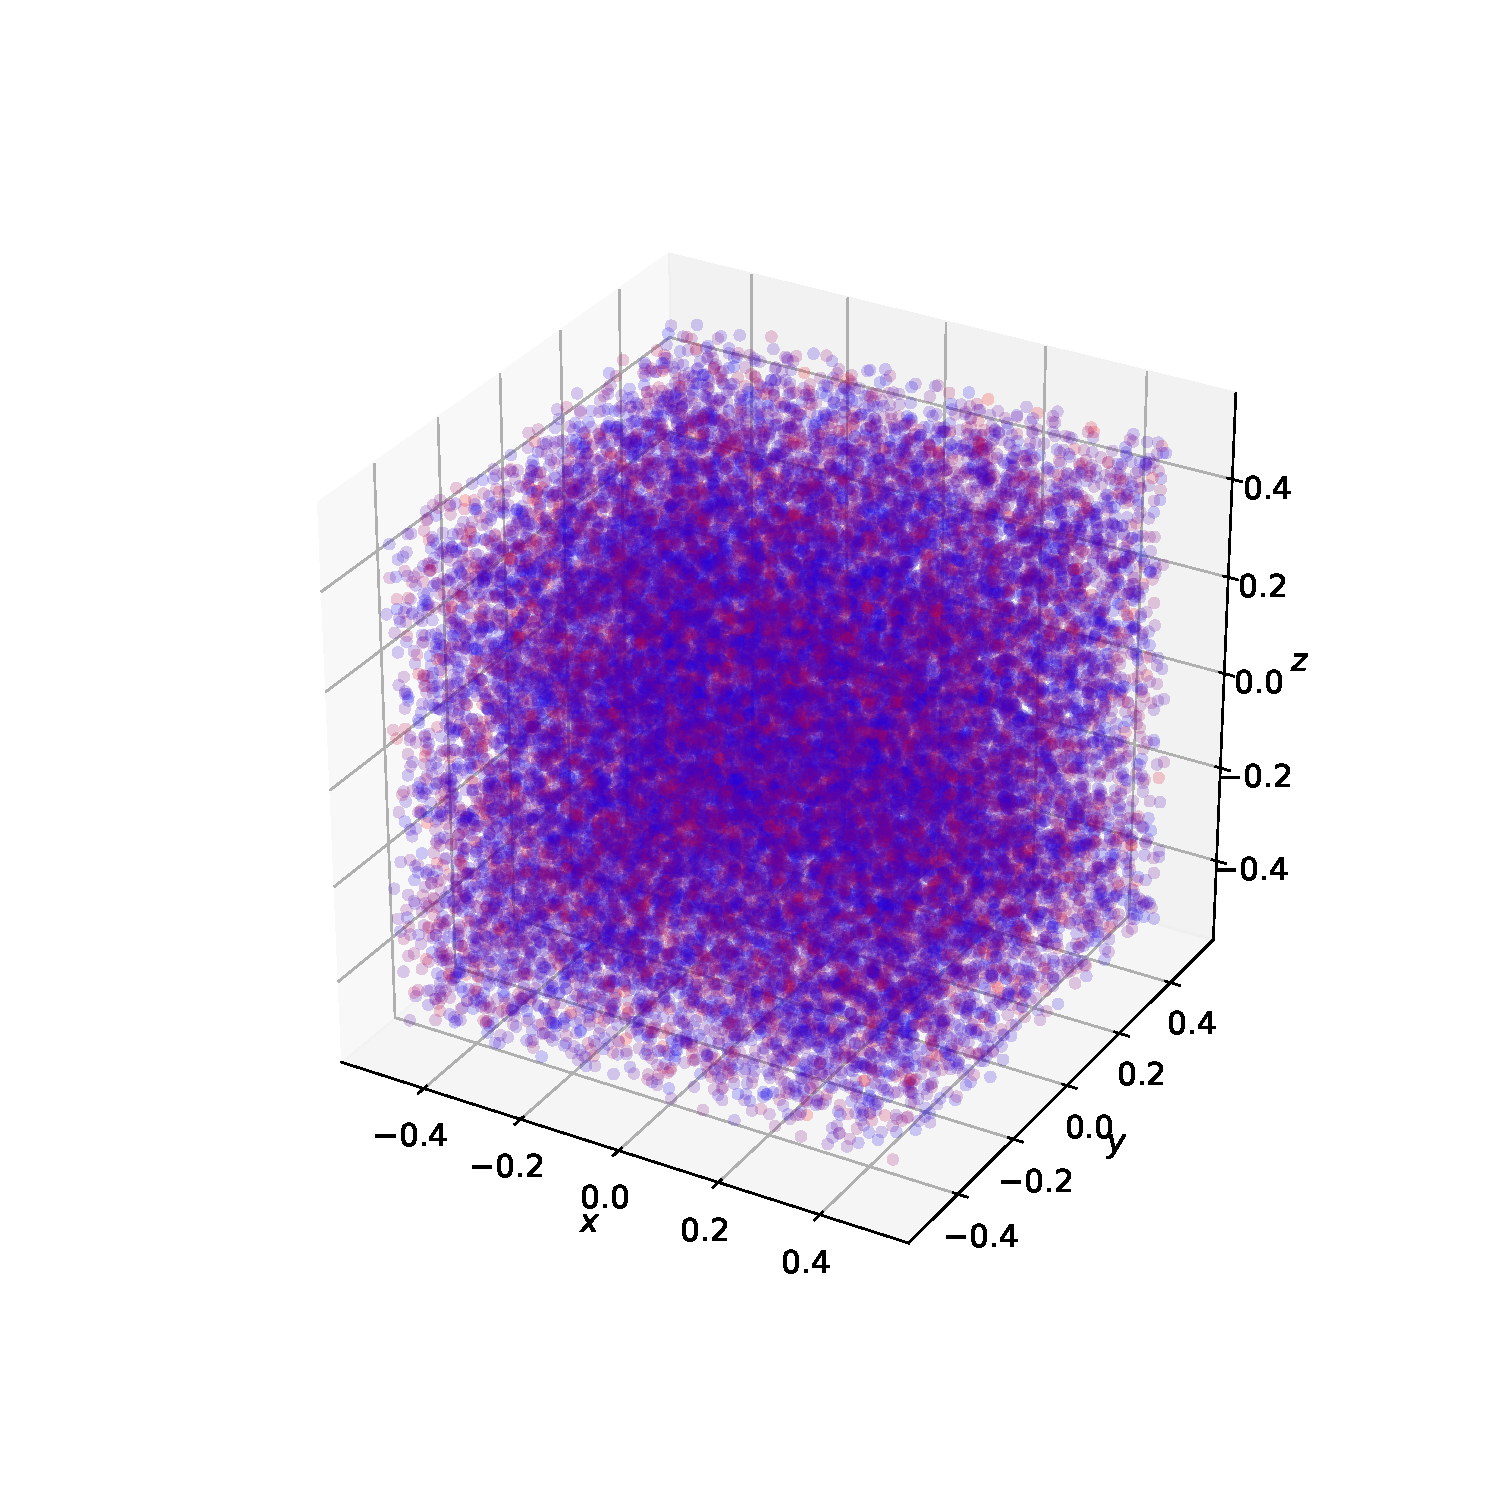
\includegraphics[width=1\linewidth]{particles}}
    \caption{Конечные положения частиц. Более красные частицы обладают большей скоростью, более синие — меньшей.}
    \end{figure}
\begin{figure}[!h]
{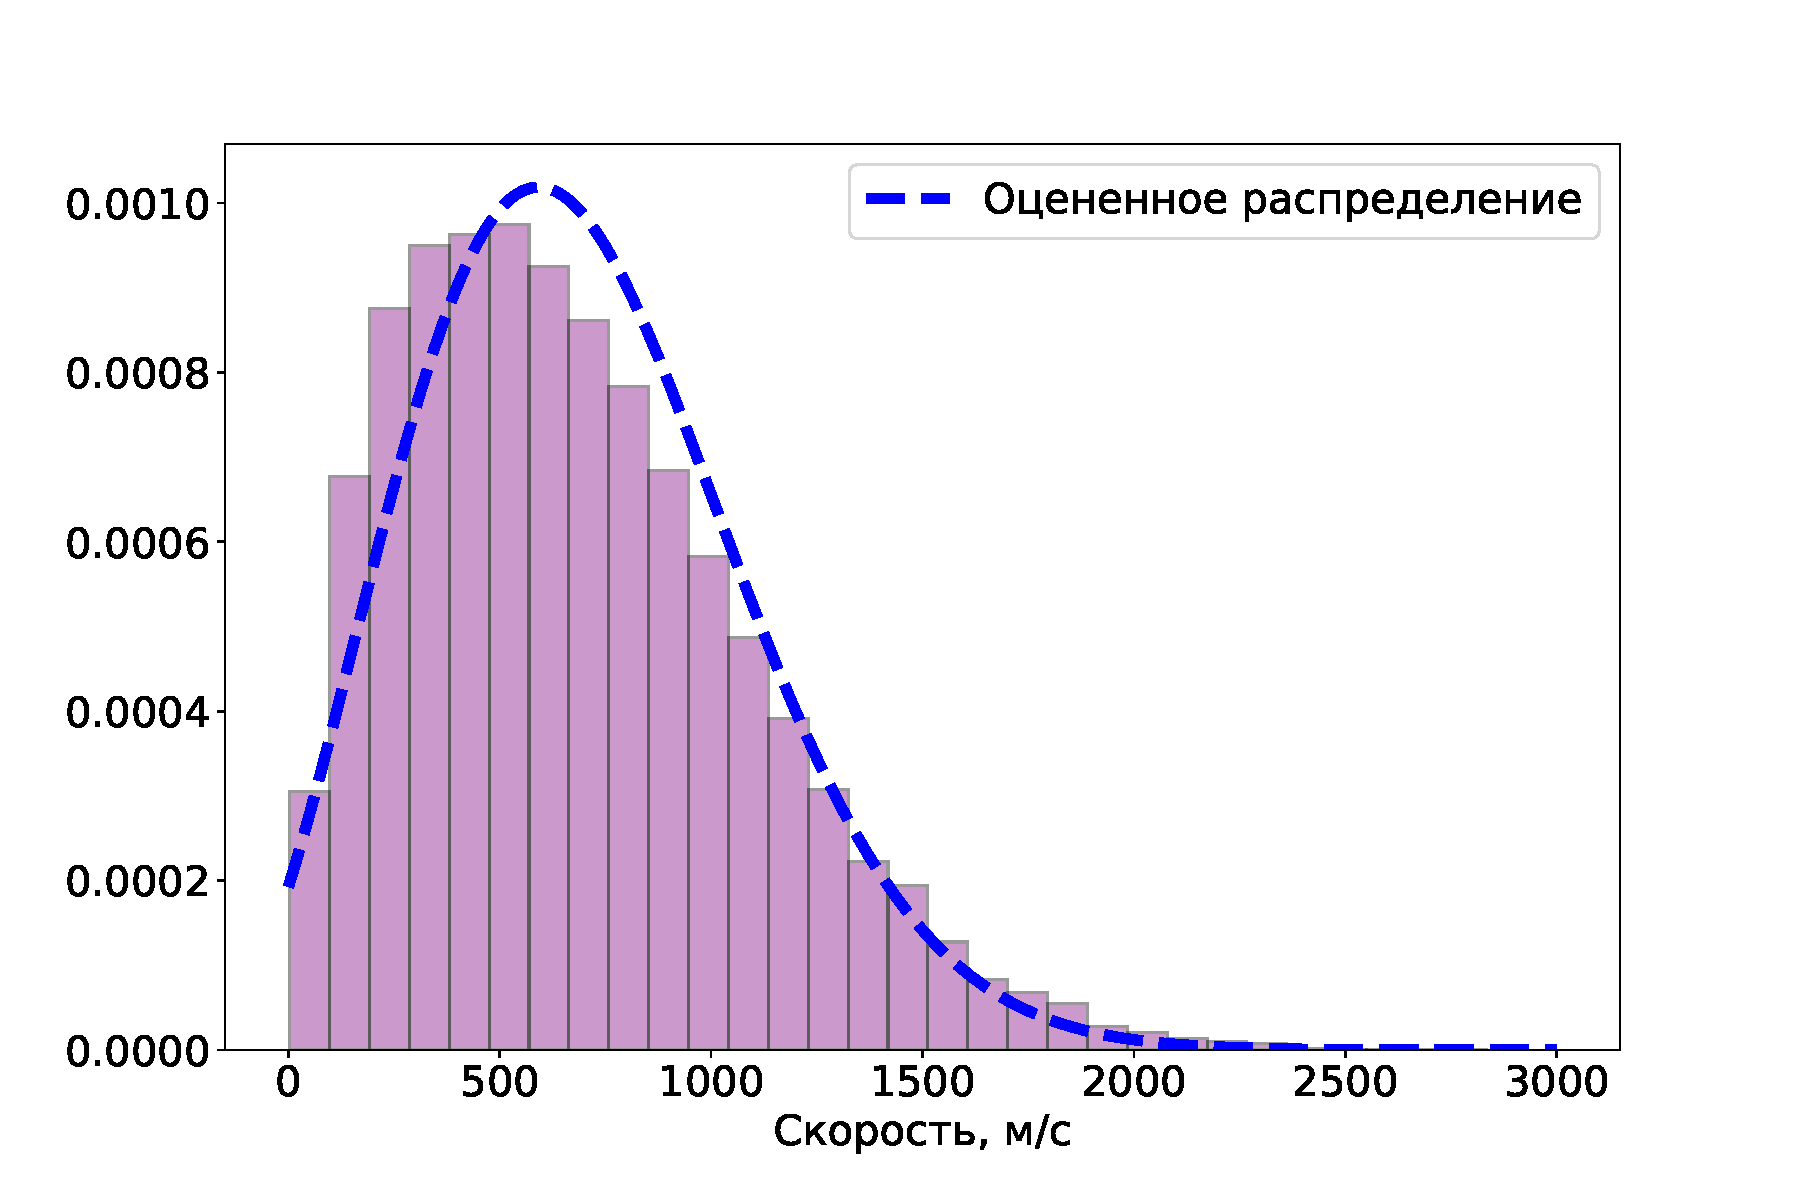
\includegraphics[width=1\linewidth]{hist_v}}
\caption{Распределение доли молекул $\Big(\dfrac{dn}{n} (\upsilon) \Big)$ по скоростям. \textit{Пунктиром} обозначено теоретическое распределение. }
\end{figure}

\indent Теоретически распределение должно иметь такую зависимость:
\begin{equation}
p(\upsilon) = 4\pi\upsilon^2 \Big( \dfrac{m}{2\pi kT} \Big)^{3/2}\cdot e^{-\dfrac{m \upsilon^2}{2kT}}
\end{equation}

\subsubsection{Проверка гипотез. Q-Q plot}
Проверим, действительно ли полученная выборка из абсолютных скоростей молекул является выборкой из распределения Максвелла. Для начала воспользуемся критерием согласия,
а именно критерием Колмогорова, критическое множество которого:
\[\sqrt{n} \cdot \sup\limits_{x \in R}{\abs{\hat{F_n}(x)- F_0(x)} > K_{1-\alpha}}. \]
Будем проверять гипотезу, что полученное распределение является распределением Максвелла с параметрами, полученными методом максимального правдоподобия. $p-value$ получившегося критерия
практически равен нулю, то есть модель все таки имеет погрешность и нельзя сказать, что полученное распределение в точности совпадает с распределением Максвелла. Получили статистически значимый результат,
но что можно сказать о его практической значимости?


\indent То, что критерий Колмогорова отверг нашу гипотезу справедливо, мы видим различие наших распределений на графиках, а с учетом размера выборки, мощность критерия практически равна единице.
Однако кажется, что распределение все равно очень близко к максвелловскому, то есть различие практически не значимо. Чтобы в этом убедиться построим часто использующийся в статистике график Q-Q plot. Чем больше он похож на прямую, тем больше похожи друг на друга выборочное и теоретическое распределения.
\begin{figure}[!h]
{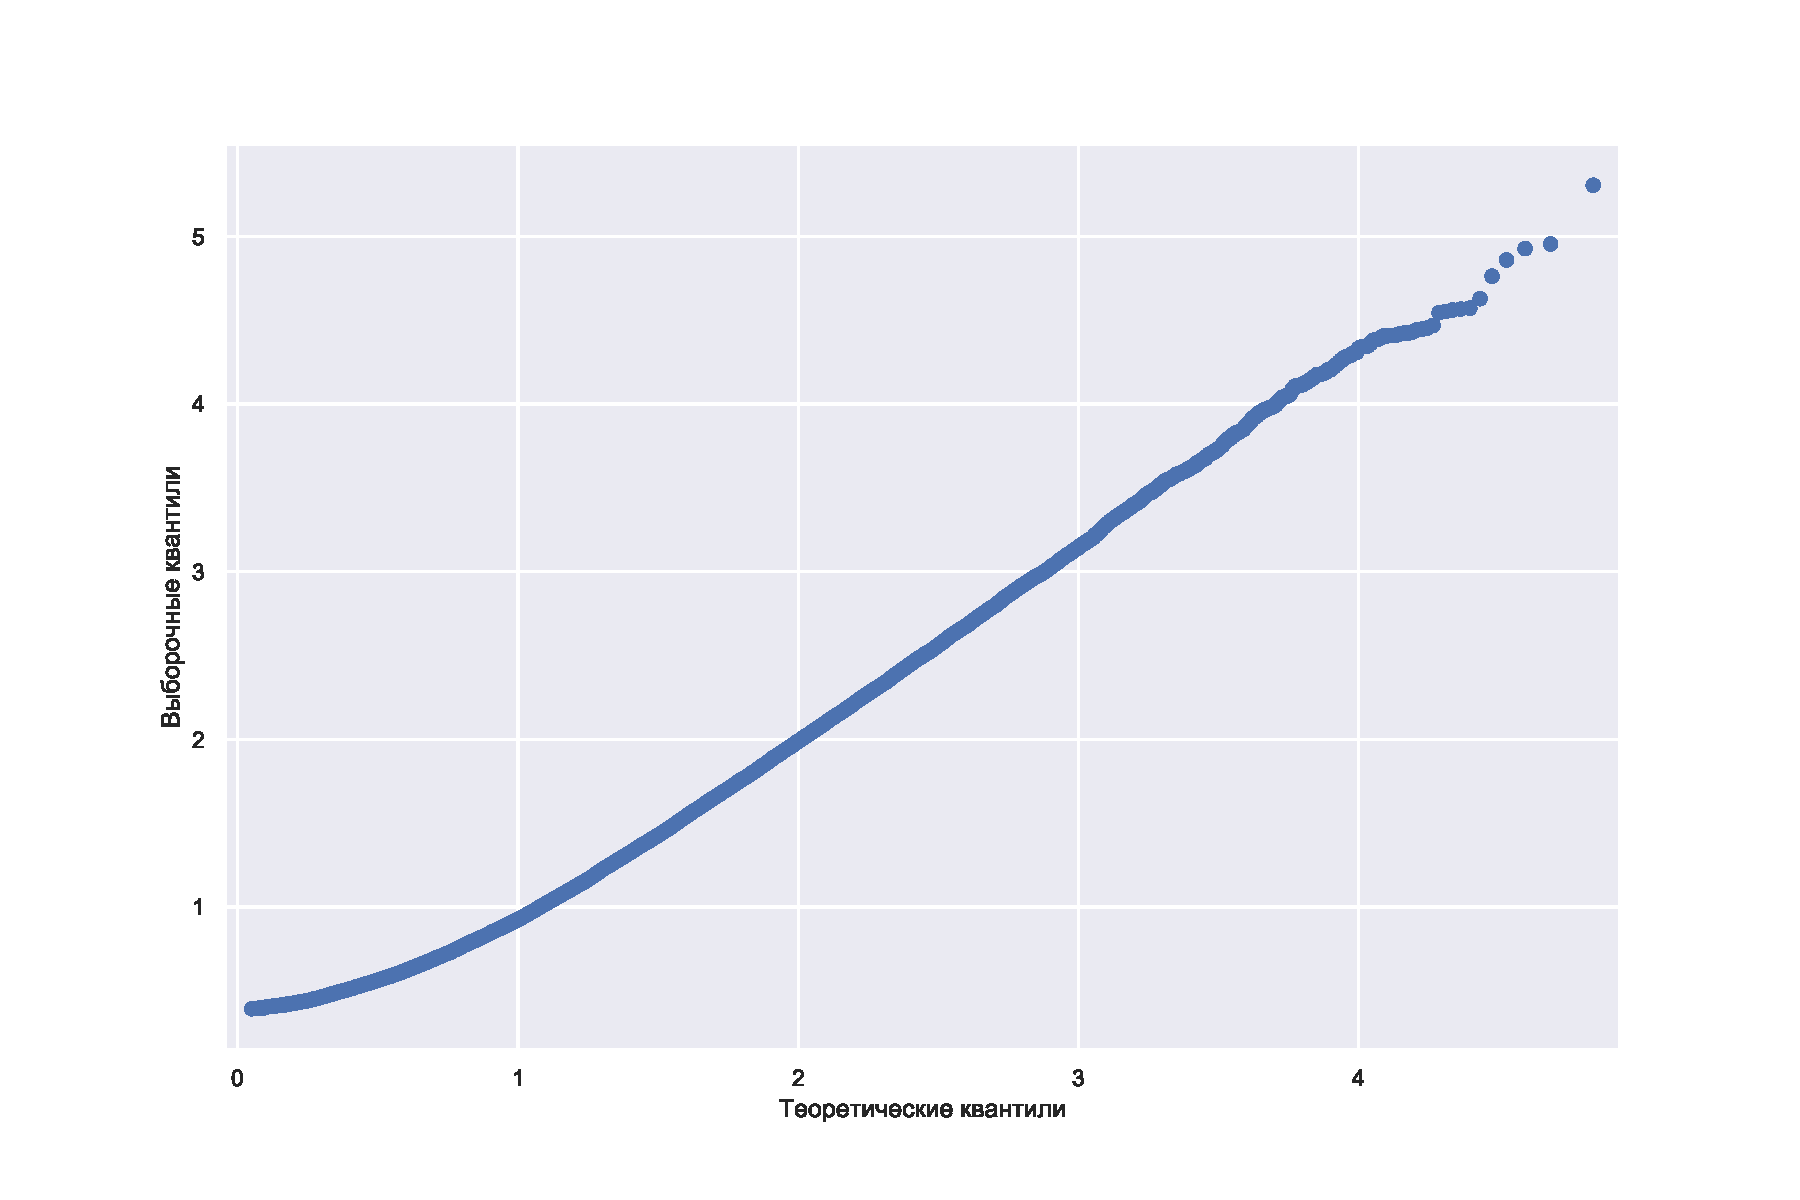
\includegraphics[width=1\linewidth]{qqplot}}
\caption{Q-Q plot}
\end{figure}


\begin{conclusion}
По графику наблюдаем, что он очень похож на прямую. Есть небольшое смещение в районе нуля, то есть по сути распределение имеет определенно максвелловский вид, незначительно завышенный в нуле.
Таким образом, с помощью Q-Q plot мы убедились, что распределение очень близко к Максвеллу.
\end{conclusion}

\subsection{Флуктуации давления}
Из курса общей физики известно, что флуктуации параметров термодинамической системы имеют вид нормального распределения.
Зачастую рассматриваются флуктуации, например, объема или температуры. Флуктуации же давления рассматривают редко, так как на
практике их практически невозможно измерить. При увеличении концентрации молекул дисперсия распределения давления в течение времени, согласно
центральной предельной теореме, имеет корневую скорость сходимости к среднему. То есть на реально получаемых концентрациях флуктуации давления
ничтожно малы. У нас же есть уникальный шанс рассмотреть эти флуктуации, так как мы просто знаем давление, а не пытаемся его измерить каким-либо прибором.
\begin{figure}[h!]
{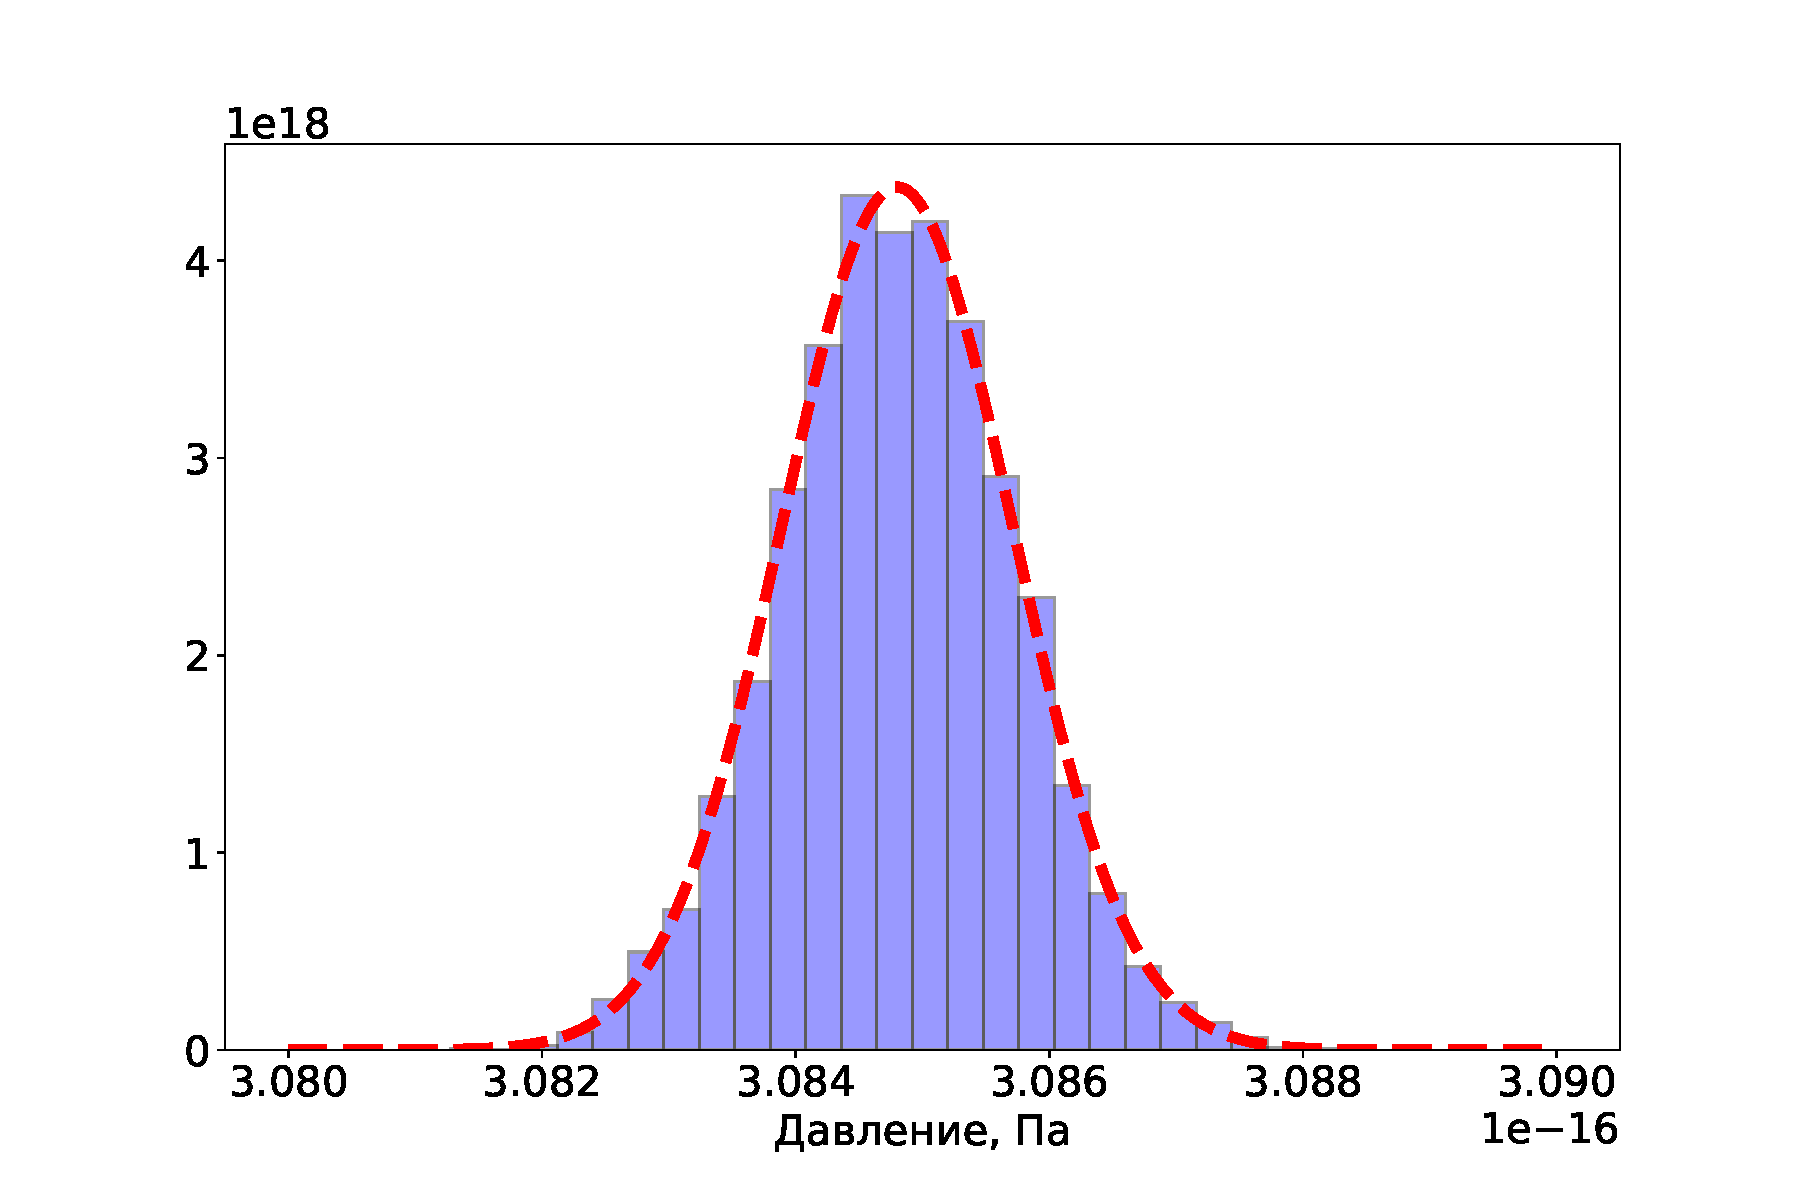
\includegraphics[width=1\linewidth]{hist_p}}
\caption{Распределение давления газа на стенки сосуда в течение времени}
\end{figure}
По графику можно заметить, что распределение точно имеет нормальный вид. Оценка по методу максимального правдоподобия дает
среднее значение $\mu = 3.0848 \cdot 10^{-16}$ Па, дисперсия $\sigma = 9.1215 \cdot 10^{-20}$ Па. Проверим гипотезу о том, что
полученная выборка действительно из этого распределения. Воспользуемся рассмотренным ранее критерием Колмогорова с уровнем
значимости $0.05$. Получаем $p-value = 0.5074 > \alpha = 0.05$, то есть гипотеза о том, что распределение давления является
нормальным распределением с параметрами $\mu$ и $\sigma^2$ не отвергалась.

\subsection{Распределение по энергиям в поле силы тяжести}

Дополнительно рассмотрим распределение энергий в поле потенциальных сил. Для примера рассмотрим систему, в которой установилось максвелловское распределение по скоростям, состоящую из 30000 частиц в кубе $1 \times 1 \times 1$ м при температуре 744.7 К, в поле силы тяжести.\\
\indent На рисунке изображена гистограмма, распределения по энергиям после 30 секунд симуляционного времени. Как можно заметить, зависимость доли частиц от энергии является экспоненциальной, и можно предположить, что она представляет из себя распределение Больцмана.

% TODO: заменить
\begin{figure}[!h]
{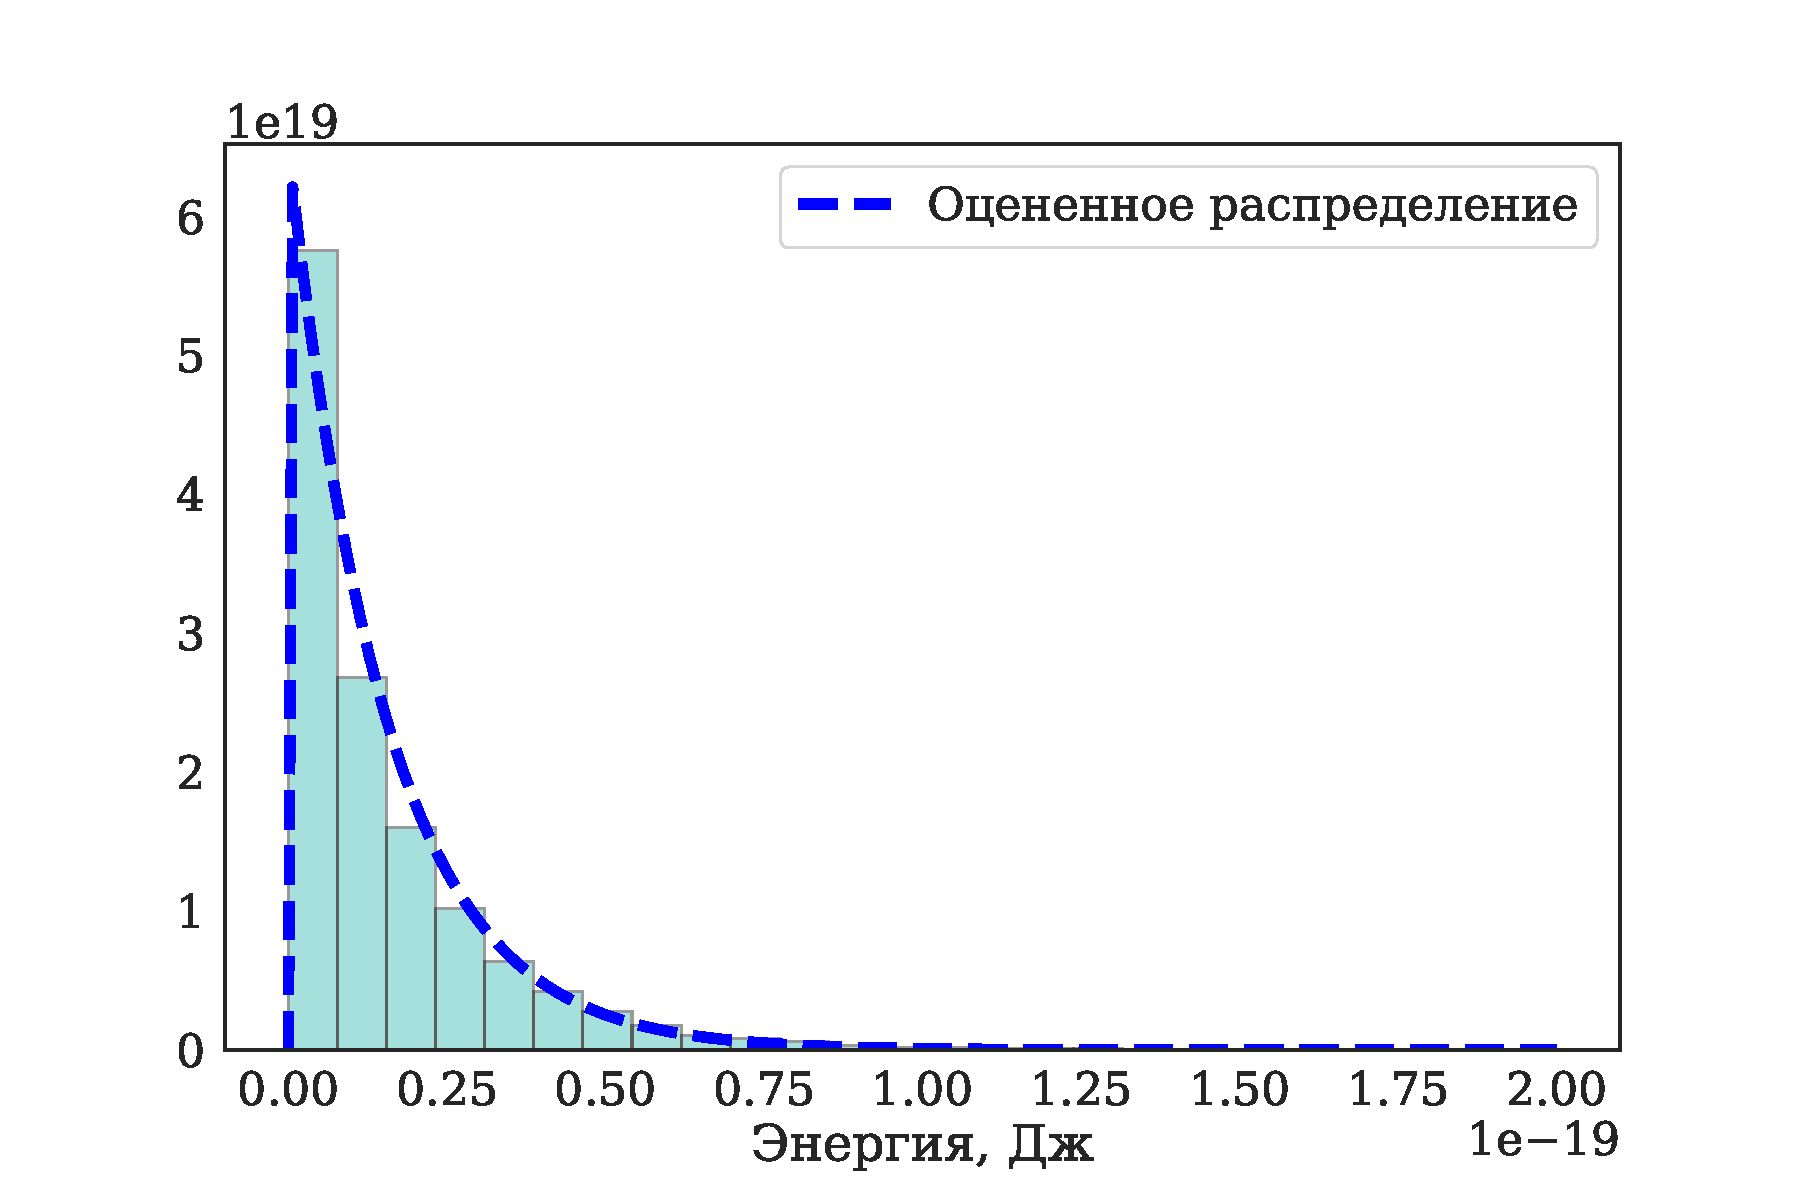
\includegraphics[width=1\linewidth]{hist_E}}
\caption{Распределение доли молекул $\Big(\dfrac{dn}{n} (\upsilon) \Big)$ по энергиям, полученное через большой промежуток времени}
\end{figure}

\subsection{Цикл тепловой машины}
Теперь, чтобы проверить выполнимость законов, описывающих изопроцессы, смоделируем следующий цикл тепловой машины:
адиабатическое сжатие (изоэнтропийный процесс), изохорное охлаждение, изотермическое расширение и изохорное нагревание.

Уравнение адиабаты для идеального газа:
\[PV^\gamma = const. \]

Тогда зная начальную точку $P_0, V_0$ не трудно построить график $P(V)$:
\[P = \dfrac{P_0 V_0^\gamma}{V ^\gamma}. \]
Т.к мы моделируем одноатомный газ, то $\gamma = \dfrac{5}{3}$.

Уравнение изотермы легко получается из равенства
$$PV = const \Rightarrow P = \dfrac{P_1 V_1}{V}.$$
\begin{figure}[!h]
{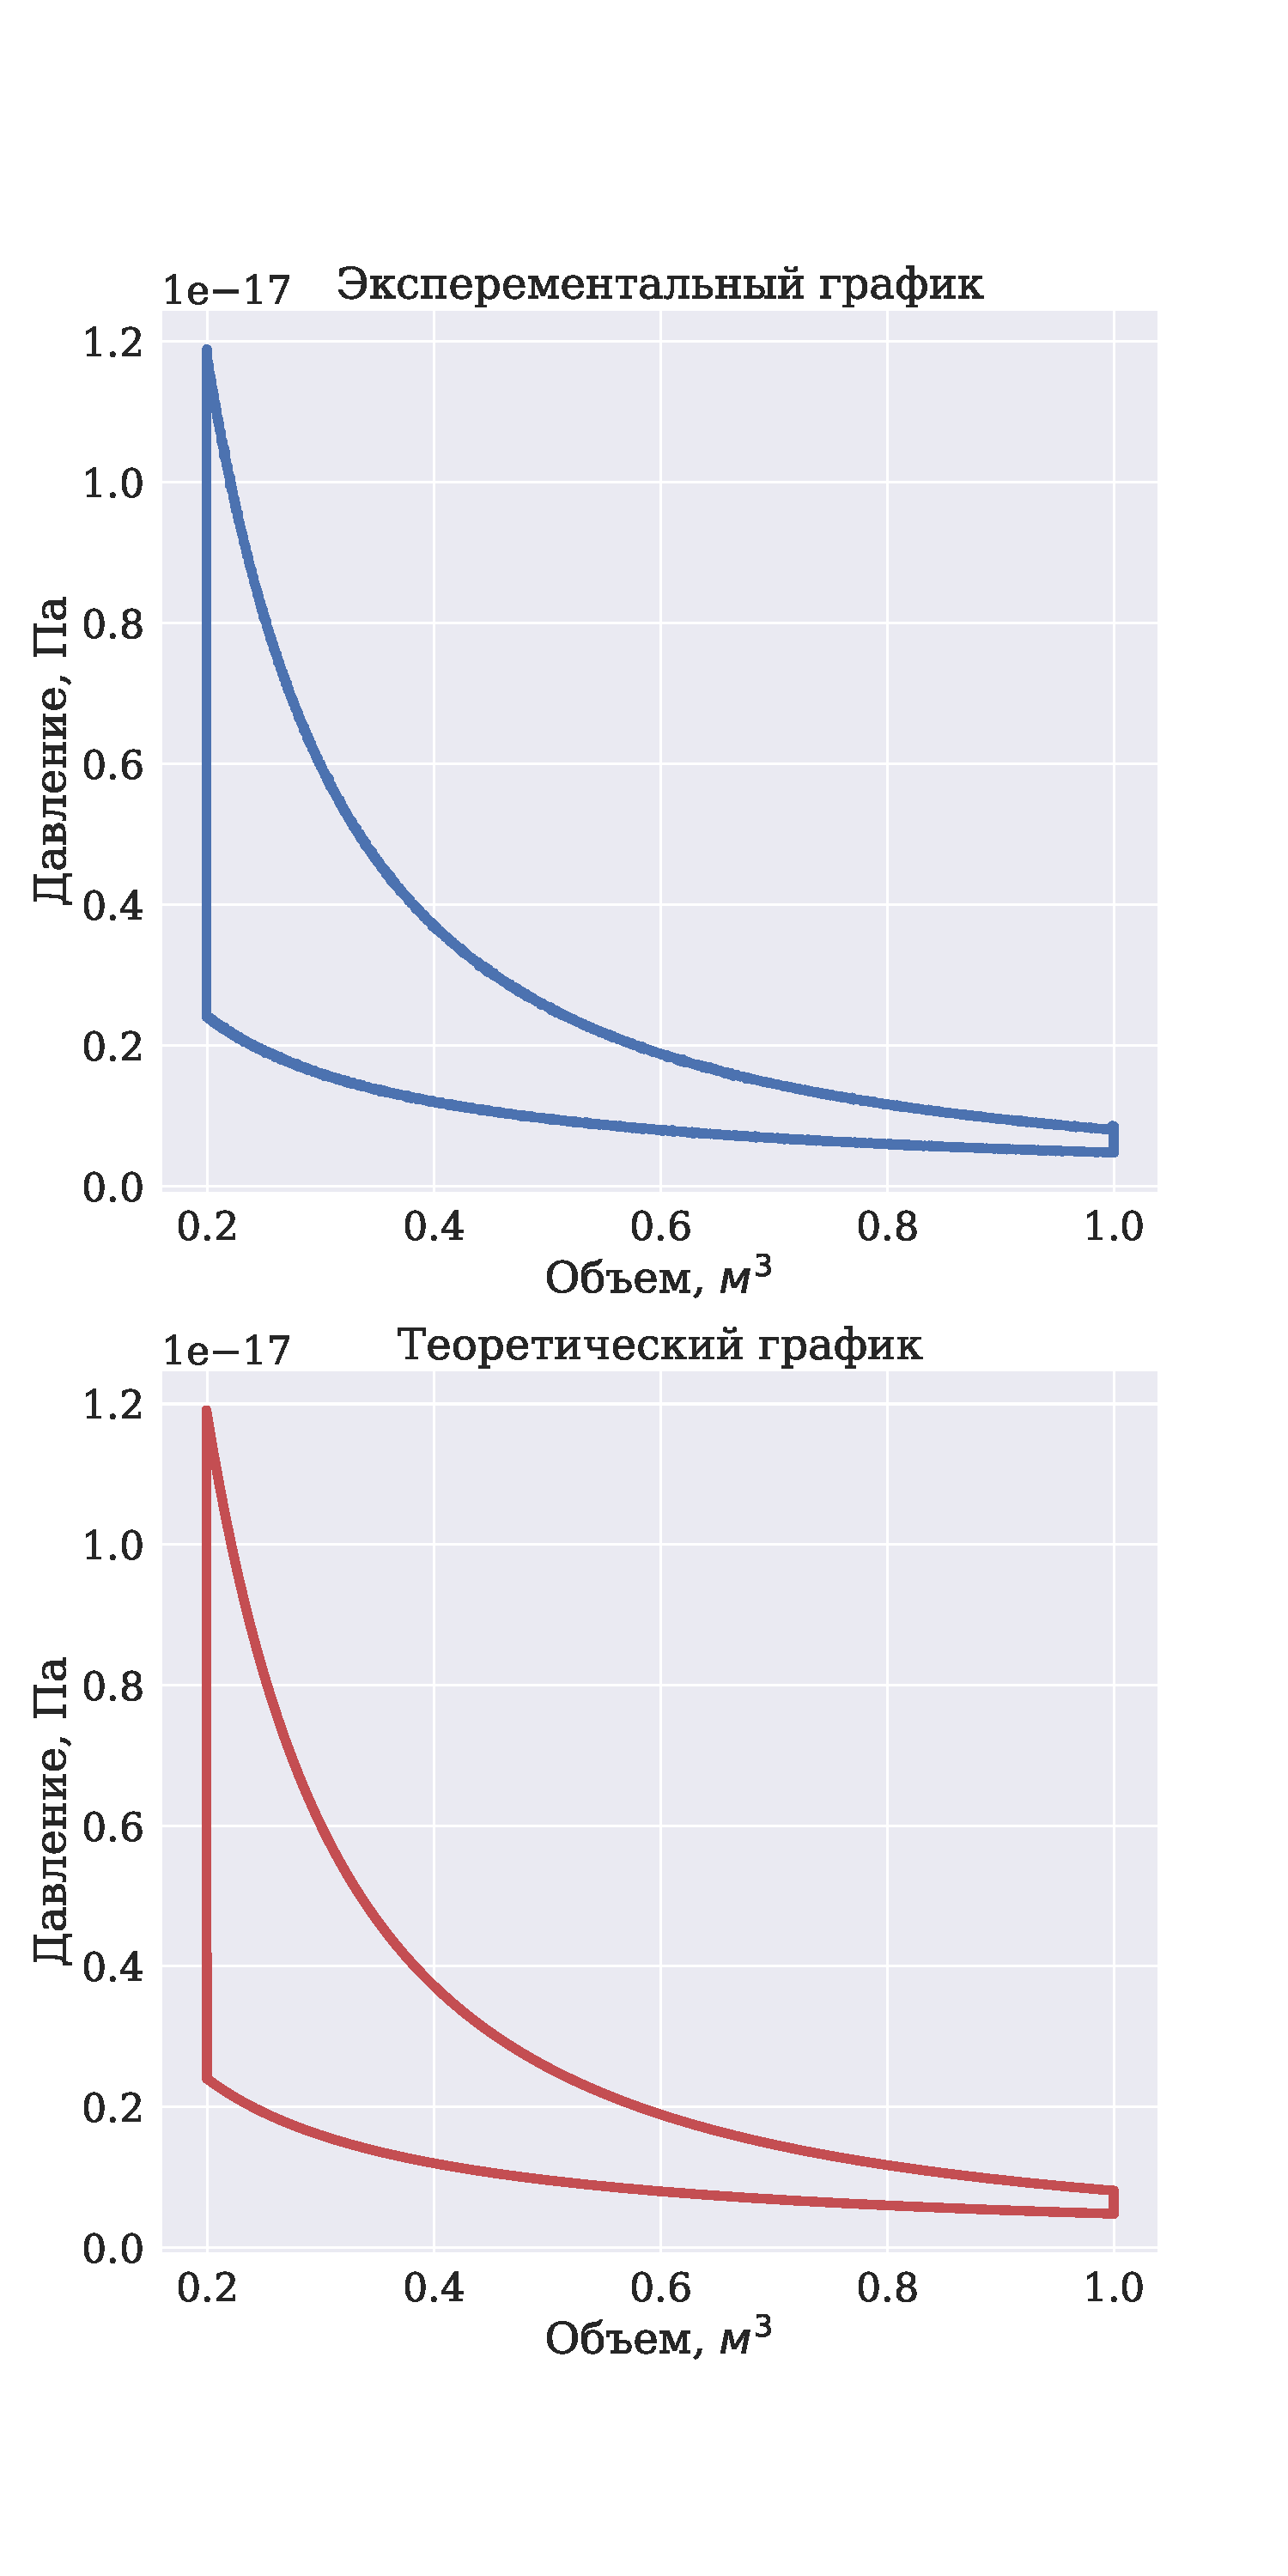
\includegraphics[width=1\linewidth]{cycle}}
\caption{Экспериментальный и теоретический графики цикла тепловой машины в $PV$ координатах.}
\end{figure}

Таким образом получили практически идеальное соответствие экспериментального и теоретического результатов, несмотря на то, что
каждый процесс был проведен в течение $10$ секунд.

\begin{conclusion}
Наша модель с высокой точностью описывает одноатомный идеальный газ. Она позволяет проводить над ним процессы и симулировать тепловую машину.
\end{conclusion}

\section{Заключение}
\indent Получили состоятельную модель идеального газа с помощью которой проверили основные законы термодинамики. Построили гипотезу о том,
что скорости молекул распределены по Максвеллу. Подтвердили нормальность флуктуаций давления. Просимулировали цикл тепловой машины.
Подводя итог, можно сказать, что действительно, симуляцией микросостояний были получены все законы, описывающие макросостояния идеального газа.

\subsection{Планы}
\begin{itemize}
\item Неидеальный газ.
Используя потенциал потенциал Леннард-Джонса $ U(z)=4 \varepsilon\left\{\left(\dfrac{\sigma}{z}\right)^{12}-\left(\dfrac{\sigma}{z}\right)^{6}\right\}$, попробовали
рассчитывать силу $F = \dfrac{dU}{dz}$.
\item Увеличение числа молекул за счет обработки столкновений только близких молекул. Оптимизация алгоритма для достижения временной сложности меньше $O(n^2)$.
\item Симуляция более сложных сосудов, смешивание газов. Отслеживание изменения энтропии.
\item Весомые поршни для проведения изобарных процессов.
\end{itemize}

%----------------------------------------------------------------------------------------
%	REFERENCE LIST
%----------------------------------------------------------------------------------------

%  ToDO: чекнуть 
\begin{thebibliography}{99} % Bibliography - this is intentionally simple in this template

\bibitem{Kirichenko:Term}
Термодинамика и статистическая физика {\em
Н.А.Кириченко, МФТИ}

\bibitem{Sivuhin:Term}
Термодинамика и Молекулярная физика {\em
Д.В Сивухин., МФТИ}

\bibitem{Modelirovanie}
Компьютерное моделирование и визуализация задач механики и
геометрии. {\em Авторы В.Л. Голо, Д.О. Синицын.}
\href{http://dfgm.math.msu.su/files/golo/modelling.pdf}{http://dfgm.math.msu.su/files/golo/modelling.pdf}

\bibitem{Sivuhin:Meh}
Механика {\em Д.В Сивухин., МФТИ}

\bibitem{Kirichenko:Meh}
Механика {\em Н.А.Кириченко, МФТИ}

\bibitem{Koriavov}
В.П. Корявов и Н.А.Кириченко. Механика
\href{https://vk.com/doc85020018_467835549?hash=d80f20a3d0b8f6643c&dl=bc29371e14b5f0ebd0}{Ссылка на выдержку}

\end{thebibliography}

%----------------------------------------------------------------------------------------

\end{document}
